%-------------------------------------------------------------------------
% Design Project Input/Output Module Description
%-------------------------------------------------------------------------

\clearpage
\section{Water Input Module}
\label{sec-input-water}

This input module enables your IoT device to sense the level of water in
the environment using a water sensor called eTape. The tape may be
secured to a street pole, hung on the wall of a room, or attached to the
side of a water container. When immersed in water, the sensor tape is
compressed from both sides by hydrostatic pressure, and the tape's
resistance varies as the water level rises and falls. The resistance and
water level are inversely proportional: the lower the water level, the
higher the output resistance; the higher the water level, the lower the
output resistance. The Arduino cannot directly sense resistance, but we
can set up a voltage divider so that the Arduino can sense voltage
instead. This way, as water level rises, the voltage the Arduino reads
rises as well.

% FIXME: replace 'ohm' with symbol..

A sample circuit and Arduino code is shown below to get you started.
The voltage divider circuit is formed by the water level sensor's middle
two leads (the outer two leads are unused) and the \wu{560}{ohm}
resistor. The Arduino reads the voltage from one end of the resistor to
ground. Use female-to-male wires to connect the water sensor to the
breadboard so that you can freely move the sensor away from the Arduino
and breadboard (which should not get wet!). The example code will print
the analog reading from the water level sensor on the serial monitor,
similar to how we printed the analog reading from the grayscale sensor
in Lab~2. After setting up the circuit and programming the Arduino, open
the serial monitor and check the value of the water level sensor when
dipped in a container of water. Try dipping the water level sensor
further into the water and make sure the reading increases.

\vspace{0.1in}
\begin{minipage}[t]{0.49\tw}
  \vspace{0pt}

  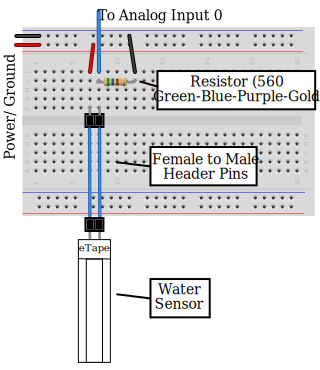
\includegraphics[width=\tw]{input-water-annotated.svg.pdf}
\end{minipage}
\hfill
\begin{minipage}[t]{0.49\tw}
  \vspace{0.1in}
  \begin{Verbatim}[gobble=3,fontsize=\small]
    int pin_water = 0;

    void setup() {
      Serial.begin(9600);
      pinMode( pin_water, INPUT );
    }

    void loop() {
      int water_level = analogRead( pin_water )

      Serial.println( water_level );
      delay(1000);
    }
  \end{Verbatim}
\end{minipage}
\vspace{0.1in}

%Questions:
